\documentclass[hyperref={pdfpagelabels=false}]{beamer}
\usepackage[T1]{fontenc}
\usepackage[latin1]{inputenc}
\usepackage[ngerman]{babel}

\usetheme{Dresden}
\usecolortheme{beaver}
%\setbeamercovered{transparent}
%\beamertemplatenavigationsymbolsempty
\setbeamertemplate{footline}[frame number]


\title{Visualisierung von Green's Function}
\author[A. Linggi, S. Steiner]{ Andreas Linggi, Stefan Steiner}

\usepackage{mathptmx}
%\usepackage[scaled=.90]{helvet}
\newcommand{\changefont}[3]{
\fontfamily{#1} \fontseries{#2} \fontshape{#3} \selectfont}
%\usefonttheme{serif}
\usefonttheme{professionalfonts}
\usepackage{tikz}
\newcommand{\red}[1]{\textcolor{red}{#1}}
%------------------- C-Code ------------------- %
\definecolor{colorkeywordstyle}{RGB}{127,0,127}
\definecolor{colorcommentstyle}{RGB}{0,116,0}
\definecolor{colorstringstyle}{RGB}{196,26,22}
\definecolor{colorbackground}{RGB}{240,240,240}
\definecolor{royalblue}{rgb}{0.15,0.25,0.55}
\definecolor{black}{rgb}{0,0,0}

\usepackage{listings}
\lstset{
  	backgroundcolor =		\color{colorbackground},
    language =				C++,			
    basicstyle =    		\ttfamily\scriptsize,
    breaklines = 			true,
    frame = 				none,
    columns =				flexible,
    keepspaces = 			true,
    keywordstyle=			\color{colorkeywordstyle},
    identifierstyle	=\color{royalblue},
    showstringspaces =		false,
    extendedchars =			true,   
    commentstyle = 			\color{colorcommentstyle},,
    numbers = 				left,
    numbersep = 			2pt,
    numberstyle =			\tiny,
    rulecolor=\color{black}, 
    stepnumber =			1,
    tabsize = 				4,
}
%---------------------------------------------


\begin{document}

\titlepage

\frame{\frametitle{Inhaltsverzeichnis}\tableofcontents} 

\section{Geschichte}

\begin{frame}
\frametitle{Geschichte} 
	\begin{itemize}[<+->]
		\item George Green
		\item 1793-1841, Nottingham
		\item Studiert in Cambridge
		\item Green's Theorem, Green's Function
		\item Partielle Differentialgleichungen
	\end{itemize}
	
	\begin{figure}
	\centering
		\pause[6] 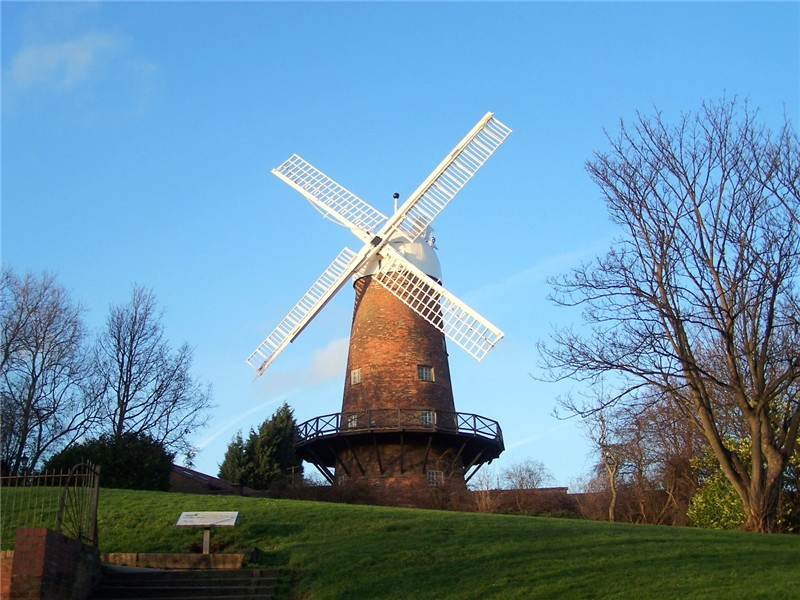
\includegraphics[width=5cm]{./images/Greens_windmill}
		\pause[7] 
\includegraphics[width=4cm]{./images/george_green_plaque2}
	\end{figure}

\end{frame}



\section{Aufgabenstellung}
Um ein Problem der Mathematik besser zu verstehen, ist es oft sehr hilfreich, wenn dieses verst�ndlich beschrieben ist. Eine Visualisierung in Form eines Bildes oder kurzen Films ist dabei eine M�glichkeit dies zu bewerkstelligen.

Die Hauptaufgabe dieses Projektes, war es nun, die Greensche Funktion in zwei Dimensionen zu visualisieren. Die L�sung f�r eine Dimension wurde bereits in einem kurzen Film veranschaulicht \footnote{\url{https://www.youtube.com/watch?v=Wpi7Gf7V2HY}}. Es soll dabei zuerst eine partielle Differentialgleichung mithilfe des Greenschen Ansatzes gel�st und danach das visualisieren umgesetzt werden. Die Greensche Funktion erm�glicht die Berechnung eines Problems durch Supperposition. Darum sollten auch verschiedene Anfangswerte untersucht werden und wie diese sich auf die L�sungen auswirken. 

Als Differentialgleichung sei dabei ein Potentialproblem vorgegeben. Vorliegend ist eine leitende Platte, die am Rande geerdet sei. Wenn nun ein Potential an einem oder mehreren Punkten auf dieser Platte anliegt, ist es von Interesse zu wissen, welches Potential man nun an einem beliebigen Punkt auf der Platte misst. Die folgende partielle Differentialgleichung l�st dabei dieses Problem.
\begin{equation}
	\dfrac{\partial^2 u}{\partial x^2}+\dfrac{\partial^2 u}{\partial y^2} = f(x,y).
\end{equation}
Dabei sei hier noch auf die Arbeit von Reto Christen und Philip Solenthaler verwiesen. Diese haben das Potentialproblem genauer untersucht. 

%\section{Grundlagen} 
\begin{frame}
\frametitle{Grundlagen} 
Die einzelnen Frames sollte einen Titel haben 
\end{frame}


\subsection{Unterkapitel von Grundlagen}
\begin{frame} 
Grundlagen bbla bla bla
\end{frame}


\section{Algorithmus}
\begin{frame}
\frametitle{Algorithmus}

\[
	A=\left(
	\begin{array}{ccccc|ccccc|c|ccccc}
	    -4&     1&     0&\cdots&     0 &     1&     0&     0&\cdots&     0 &\cdots &      &      &      &      &      \\
	     1&    -4&     1&\cdots&     0 &     0&     1&     0&\cdots&     0 &\cdots &      &      &      &      &      \\
	     0&     1&    -4&\cdots&     0 &     0&     0&     1&\cdots&     0 &\cdots &      &      &     0&      &      \\
	\vdots&\vdots&\vdots&\ddots&\vdots &\vdots&\vdots&\vdots&\ddots&\vdots &       &      &      &      &      &      \\
	     0&     0&     0&\cdots&    -4 &     0&     0&     0&\dots &     1 &\cdots &      &      &      &      &      \\
	\hline
	     1&     0&     0&\cdots&     0 &    -4&     1&     0&\dots &     0 &\cdots &      &      &      &      &      \\
	     0&     1&     0&\cdots&     0 &     1&    -4&     1&\dots &     0 &\cdots &      &      &      &      &      \\
	     0&     0&     1&\cdots&     0 &     0&     1&    -4&\dots &     0 &\cdots &      &      &     0&      &      \\
	\vdots&\vdots&\vdots&\ddots&\vdots &\vdots&\vdots&\vdots&\ddots&\vdots &       &      &      &      &      &      \\
	     0&     0&     0&\cdots&     1 &     0&     0&     0&\cdots&    -4 &\cdots &      &      &      &      &      \\
	\hline
	\vdots&\vdots&\vdots&      &\vdots &\vdots&\vdots&\vdots&      &\vdots &\ddots &\vdots&\vdots&\vdots&      &\vdots\\
	\hline
	      &      &      &      &       &      &      &      &      &       &\cdots &    -4&     1&     0&\cdots&     0\\
	      &      &      &      &       &      &      &      &      &       &\cdots &     1&    -4&     1&\cdots&     0\\
	      &      &     0&      &       &      &      &     0&      &       &\cdots &     0&     1&    -4&\cdots&     0\\
	      &      &      &      &       &      &      &      &      &       &       &\vdots&\vdots&\vdots&\ddots&\vdots\\
	      &      &      &      &       &      &      &      &      &       &\cdots &     0&     0&     0&\cdots&    -4\\
	\end{array}
	\right) 
	\]

\end{frame}
\section{Parallelisierung}

\begin{frame}
\frametitle{Parallelisierung} 
	\begin{itemize}[<+->]
		\item OpenMP
		\item \lstinputlisting{./parallel_for.c}
		\item Ein gemeinsamer Speicher
		\item Gauss-Seidel und OpemMP
	\end{itemize}
\end{frame}

\begin{frame}
	\centering
	Nach dem ersten Schritt mit 32 Threads:
	
	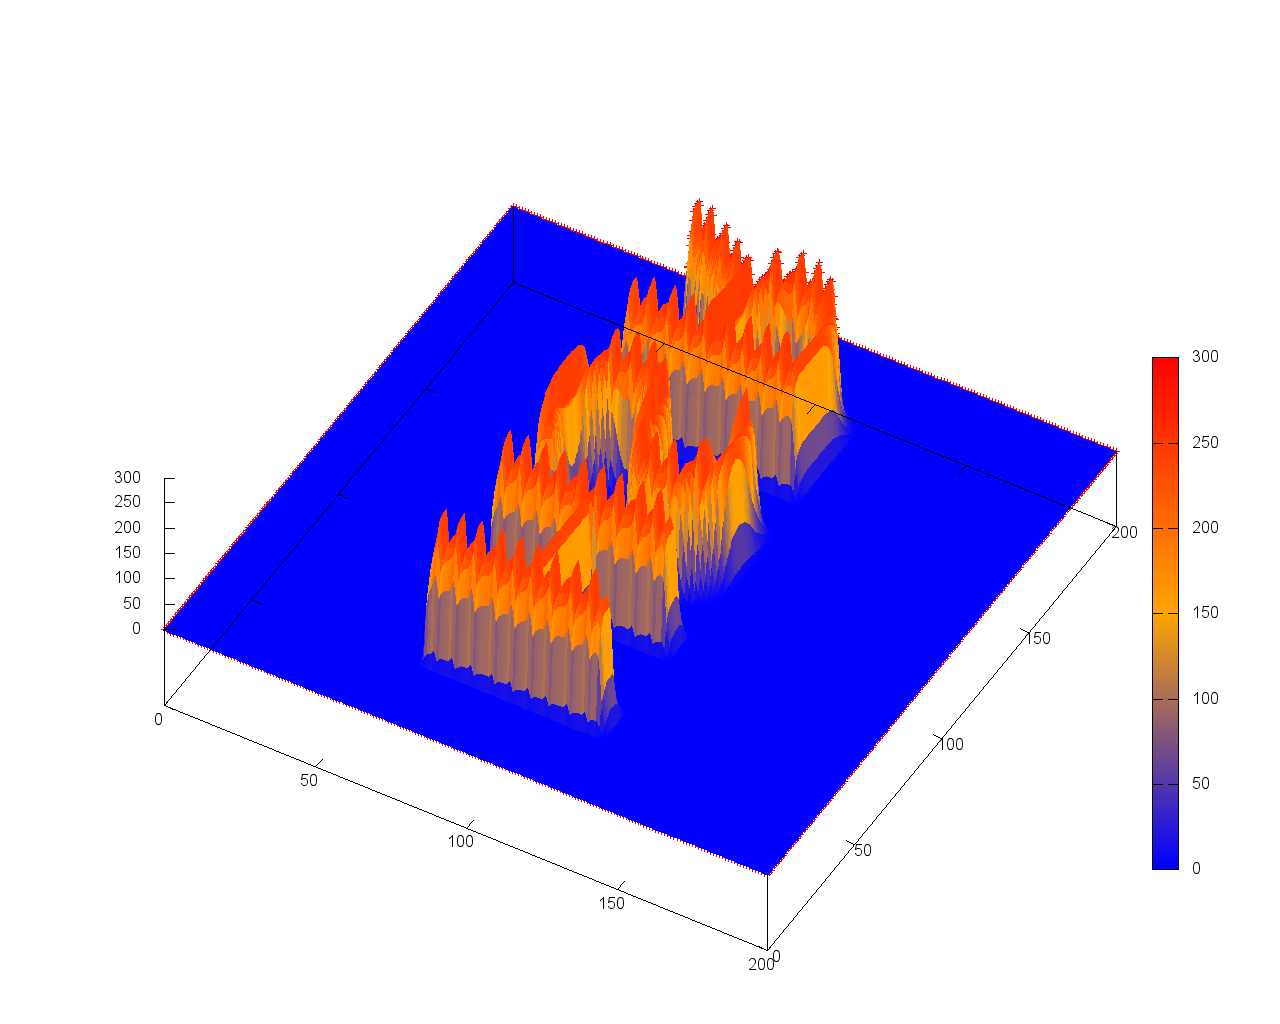
\includegraphics[width = 10cm]{../skript/images/step001}
\end{frame}




\section{FITS-File}
\begin{frame}
\frametitle{FITS-File}
\begin{itemize}
\item  Einf\"uhrungskurs in \LaTeX{} \pause 
\item  Kurs 2 \pause 
\item  Seminararbeiten und Pr\"asentationen mit \LaTeX{} \pause 
\item  Die Beamerclass
\end{itemize} 
\end{frame}
\section{Visualisierung}
	
	Wir speichern die erhaltene Matrix in einem .csv File mit einer Genauigkeit von vier Nachkommastellen ab, was f�r eine Visualisierung absolut hinreichen ist. Anfangs benutzten wir MATLAB um aus dem CSV-File eine anst�ndige Visualisierung zu erhalten. Der Aufwand war gering und die Resultate waren schnell kontrollierbar.
	
	\lstinputlisting{./csvToMatrixAndPlot.m}
	
	Um das zu automatisieren benutzen wir sp�ter Gnuplot, welches sich mit C-Code ohne Probleme ansprechen l�sst und uns die Bilder automatisch mit dem vorgegebenen Einstellungen erstellt.
	
	Gnuplot ist ein Kommandozeilen basiertes OpenSource Tool, das aber auch mit GUI erh�ltlich ist. �ber eine Pipe lassen sich lassen sich alle Einstellungen vornehmen und aus dem .CSV-File ein PNG generieren.
	
	\lstinputlisting{./gnuplot.c}
	
	Mit der Green-Funtion k�nnen bei einer partiellen DGL 2. Ordnung einzelne Punkte berechnet werden. Um das zu visualisieren, berechnen wir einzelne Ringe bzw. Quadrate vom Zentrum ausgehen nach aussen. Man k�nnte nat�rlich auch jeder Punkt einzeln dazu nehmen, was mehr Berechnungen erfordert.
	
		\[
			f=\left(
			\begin{array}{ccccc}
			    f_{11}& f_{12}& f_{13}& f_{14}& f_{15}\\
				f_{21}& f_{22}& f_{23}& f_{24}& f_{25}\\
				f_{31}& f_{32}& \red{f_{33}}& f_{34}& f_{35}\\
				f_{41}& f_{42}& f_{43}& f_{44}& f_{45}\\
				f_{51}& f_{52}& f_{53}& f_{54}& f_{55}\\
			\end{array}
			\right) \Rightarrow
			\left(
			\begin{array}{ccccc}
			    f_{11}& f_{12}& f_{13}& f_{14}& f_{15}\\
				f_{21}& \red{f_{22}}& \red{f_{23}}& \red{f_{24}}& f_{25}\\
				f_{31}& \red{f_{32}}& \red{f_{33}}& \red{f_{34}}& f_{35}\\
				f_{41}& \red{f_{42}}& \red{f_{43}}& \red{f_{44}}& f_{45}\\
				f_{51}& f_{52}& f_{53}& f_{54}& f_{55}\\
			\end{array}\right)
			\Rightarrow
			\left(\red{
			\begin{array}{ccccc}
			    f_{11}& f_{12}& f_{13}& f_{14}& f_{15}\\
				f_{21}& f_{22}& f_{23}& f_{24}& f_{25}\\
				f_{31}& f_{32}& f_{33}& f_{34}& f_{35}\\
				f_{41}& f_{42}& f_{43}& f_{44}& f_{45}\\
				f_{51}& f_{52}& f_{53}& f_{54}& f_{55}\\
			\end{array}}
			\right)
			\]

	
	Diese einzelnen Schritte werden vollst�ndig berechnet und dann als .csv abgespeichert. Die Bilder werden nachdem alle Einzelschritte berechnet wurden aus den Dateien wiederum parallelisiert in einer \verb|for|-Schleife zu .png Bilddateien verarbeitet. Die Skalierung der z-Achse wird direkt aus den Daten des letzten Schrittes berechnet, was uns eine optimale Darstellung garantiert. Aus den Bilddateien wird am Schluss optional noch ein Video erstellt.
		
\section{Probleme}
	
	Die Fl�che $f$ kann alle m�glichen Werte als Anfangsbedingung haben. Wir haben anfangs den  HSR-Schriftzug als FITS-File in eine Matrix 
	eingelesen. Der maximale Wert betrug anfangs nur 255,
	stieg nach einigen hundert Iterationen auf �ber 3000 an und die Funktion nahm die Form eines Haufen an. Wir hatten mit einem anderem Resultat gerechnet und �berpr�ften unseren Algorithmus. Wir konnten keinen Fehler entdecken und konnten die Werte mit MATLAB verifizieren. Die n�chste Frage war, ob der Gauss-Seidel konvergiert. Wir berechneten den Spektralradius der Matrix $A$ gem�ss Definition\;5.1 aus dem Skript HPC:
	
	\begin{eqnarray}
		A = M+N\\
		\varrho(M^{-1}N)<1
	\end{eqnarray}
	
	Da die Berechnung schnell sehr rechenaufwendig wird, man beachte, dass die Gr�sse der Matrix $A$ mit $n^4$ zunimmt, haben wir Matrizen mit kleinem $n$ berechnet. 	
	
	\begin{table}[h]
		\begin{tabular}{cc}
			n & Specktralradius $\varrho$\\\midrule
			5 & 0.7500\\
			10 & 0.92063\\
			15 & 0.96194\\
			20 & 0.97779\\
			25 & 0.98547\\
			40 & 0.99414
		\end{tabular}
		\centering
		\caption{Spaktralradien der Matrix $A$ f�r eine Matrix $f$ mit der Gr�sse $n\times n$}
	\end{table}

	Einerseits sind alle Werte kleiner Eins, was gut ist, andererseits sind die Werte sehr nahe bei Eins, was erkl�rt wieso unser Algorithmus so langsam konvergiert.
	
	Wir hatten sp�ter Erfolge, wenn wir die Anfangswert der Matrix $f$ klein w�hlten $(f_{ij}<1)$. So waren die Fehler von Anfang an kleiner und wir bekamen brauchbare Werte.
	
	Bei gr�sseren Matrizen mussten wir darauf achten, dass wir nicht zu viele Daten abspeichern. Wir mussten das Programm so umschreiben, dass wir einstellen konnten wie viele Bilder wir schlussendlich wollten. Anhand von diesem Einstellungen wurde nur die ben�tigten .csv und .png Dateien abgespeichert. Das Programm wurde dadurch automatisch auch gleich viel schneller. 
\section{Demonstration}
	
\begin{frame}
\centering\huge Demostartion
\end{frame}

\begin{frame}
\centering\huge Fragen?
\end{frame}


	
\end{document}